\chapter{Implementation of the MARVIS System}

Transitioning a designed system into a fully operational, real-time surveillance framework demands strict integration of disparate processing modules, software libraries, and hardware resources. This chapter details how the architectural decisions outlined previously were practically executed to construct a unified pipeline capable of live vessel monitoring and trajectory forecasting. 

Rather than building the system as a monolithic application, I adopted a modular implementation strategy. Each component—ranging from video ingestion to sensor fusion—was developed, configured, and tested in isolation. This approach made it significantly easier to trace bugs and optimize performance before bringing the entire pipeline online. The following sections detail the environment configuration, data preparation, model training, and the final assembly of the functional modules.

\section{Top-Level System Implementation}

At the highest level, the implementation relies on a pipeline architecture where each stage operates independently but communicates via strictly defined data interfaces. This prevents a bottleneck in one area (such as the computationally heavy trajectory prediction) from crashing the real-time video feed. 

The framework is divided into six primary stages: video ingestion, ship detection, multi-object tracking, sensor fusion, trajectory prediction, and geospatial visualization. Figure~\ref{fig:deployment} illustrates how these modules are deployed and how data flows between them in the backend environment.

\begin{figure}[H]
\centering
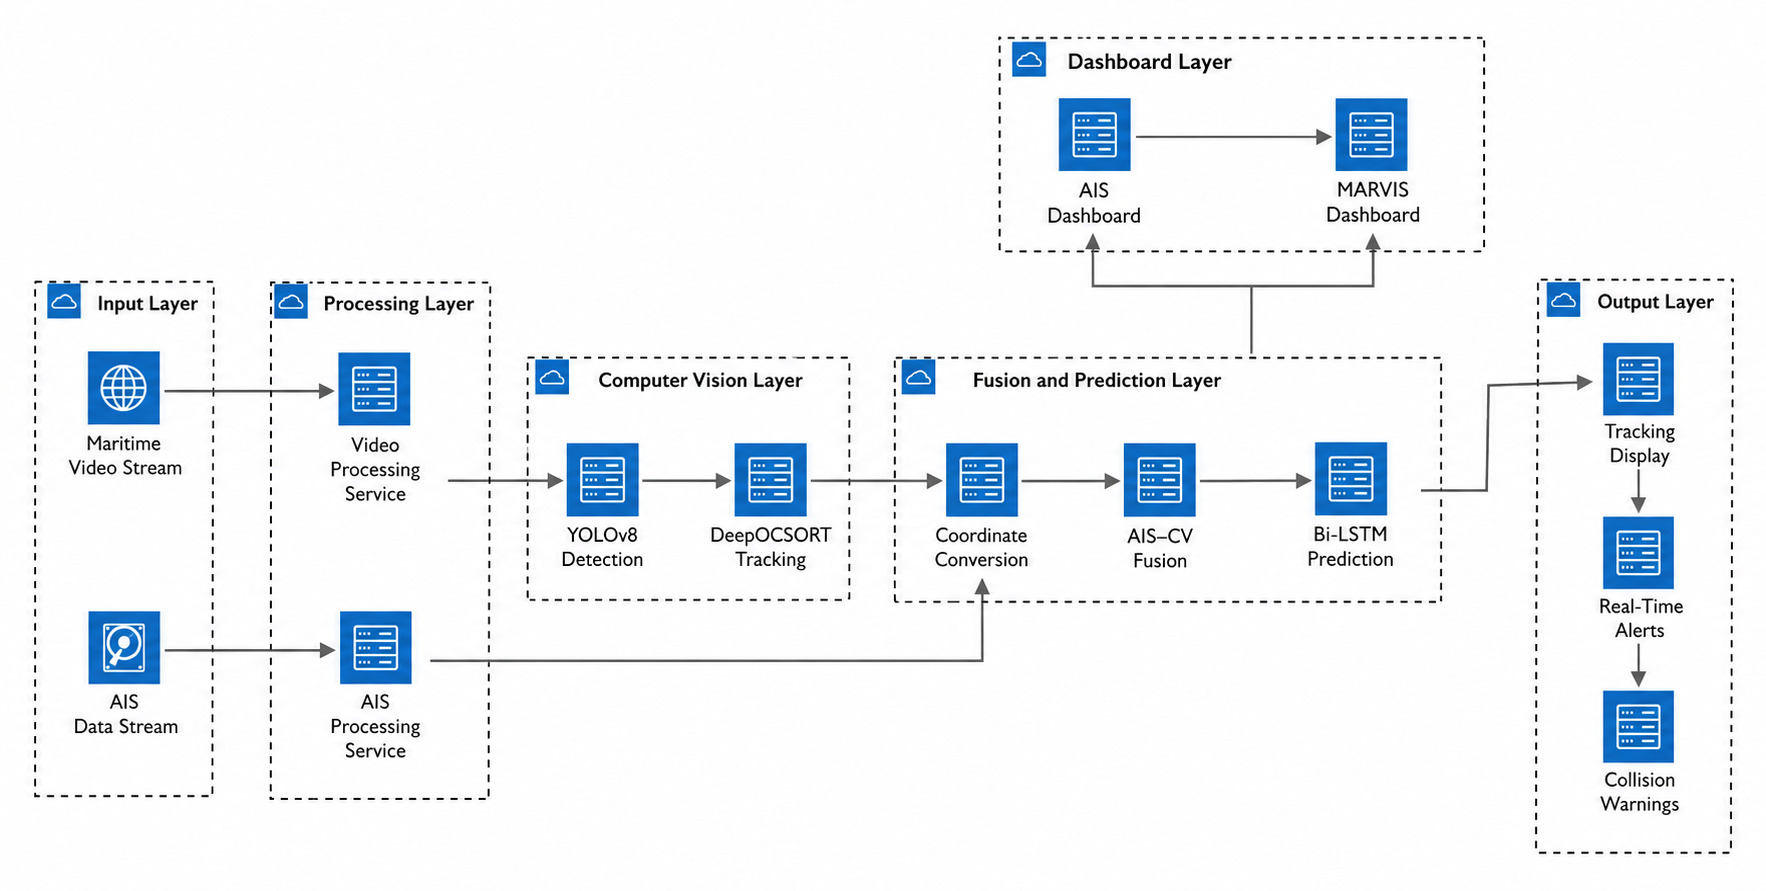
\includegraphics[width=0.95\textwidth]{Chapter4/Figures/deployment_architecture.jpeg}
\caption{Deployment and Backend Communication Architecture of Proposed Maritime Surveillance System}
\label{fig:deployment}
\end{figure}

\subsection{Development Environment Configuration}

The core logic was written in Python 3.8, selected primarily for its deep ecosystem of machine learning libraries. Deep learning operations—specifically the \gls{yolov8} detector and the \gls{lstm} forecasting network—were implemented using \gls{pytorch}. 

For the vision pipeline, \gls{opencv} handled all video ingestion, frame-by-frame extraction, and the rendering of bounding boxes onto the live feed. In the background, NumPy and Pandas managed the intermediate data structures, such as the arrays holding centroid coordinate histories and the sequence buffers required by the neural networks. Visualization was split between Matplotlib for offline analytical plotting and Folium for rendering the live, interactive geographical maps.

Crucially, the entire pipeline was deployed on an \gls{nvidia} \gls{gpu}-enabled environment utilizing \gls{cuda} acceleration. Without hardware acceleration, running simultaneous deep learning detection, appearance tracking, and sequence prediction at 30 frames per second would be computationally impossible. Primary development and debugging were conducted via Visual Studio Code and Jupyter Notebooks.

\subsection{Data Preparation and Model Training}

Before integrating the vision models into the real-time pipeline, they required extensive training. The raw maritime video data was parsed into individual frames at a fixed sampling interval, generating a robust dataset that captured diverse sea states, lighting conditions, and vessel occlusions. These frames were annotated with \gls{yolo}-formatted bounding boxes that recorded the class identifier alongside the normalized center coordinates, width, and height of every visible ship. 

To prevent overfitting, the dataset was split into training, validation, and testing partitions using a 70:20:10 ratio. During the training phase, several augmentation techniques—including horizontal flipping, mosaic augmentation, random cropping, and brightness jittering—were dynamically applied to force the model to generalize across unpredictable maritime environments.

For the detection module, \gls{yolov8} was initialized with pretrained COCO weights and then fine-tuned via transfer learning. The training process utilized a Stochastic Gradient Descent (SGD) optimizer combined with a Cosine Annealing learning rate scheduler. Early stopping was implemented, halting training once the mean Average Precision (mAP) on the validation set ceased to improve. For live inference, the model was strictly constrained by a confidence threshold of 0.5 and a \gls{nms} \gls{iou} threshold of 0.45. Any bounding box prediction falling below this confidence level is immediately discarded, ensuring that the downstream tracker isn't overwhelmed by false positives.

Following detection, the confirmed bounding boxes are passed to the \gls{deepocsort} multi-object tracking module. The tracker was configured with a maximum track age of 30 frames and requires at least 3 consecutive hits to confirm a new track. To handle identity preservation, \gls{deepocsort} utilizes an \gls{osnet} feature extractor to generate compact visual embeddings of each ship. During execution, it first attempts to match new detections to existing tracks based on spatial overlap (\gls{iou}). If that fails—often due to vessels crossing paths—it compares the \gls{osnet} embeddings using cosine similarity to successfully re-identify the ship based on its appearance. Active track coordinates are subsequently stored in a rolling buffer for motion analysis.

\subsection{Motion Estimation and Sensor Fusion}

By maintaining a historical buffer of centroid coordinates for every active track, the system can continuously calculate inter-frame motion parameters. Instantaneous speed is derived from the Euclidean distance traveled across consecutive frames, while the vessel's heading is extracted from the horizontal and vertical displacements using standard trigonometric relationships. For operator clarity, these precise angular headings are mapped to cardinal and intermediate directions before being overlaid onto the live video feed.

In parallel, the sensor fusion module ingests the live \gls{ais} telemetry stream, containing critical metadata like the \gls{mmsi}, absolute geographical coordinates, \gls{sog}, and \gls{cog}. To merge these disparate data sources, the pixel coordinates of the tracked ships are projected into geographic coordinates via a homographic transformation. The system then calculates the Haversine distance between the camera-derived coordinates and the \gls{ais} reports, employing a nearest-neighbor approach to link them. 

Once associated, the visual track is appended with the \gls{ais} metadata. However, because camera projections are inherently noisy, a Kalman filter is applied to the fused state. This filter leverages the high-frequency visual updates against the sparse but accurate \gls{ais} telemetry to produce a highly stable, real-time estimate of the vessel's actual position and velocity (Figure~\ref{fig:fusion}).

\begin{figure}[H]
\centering
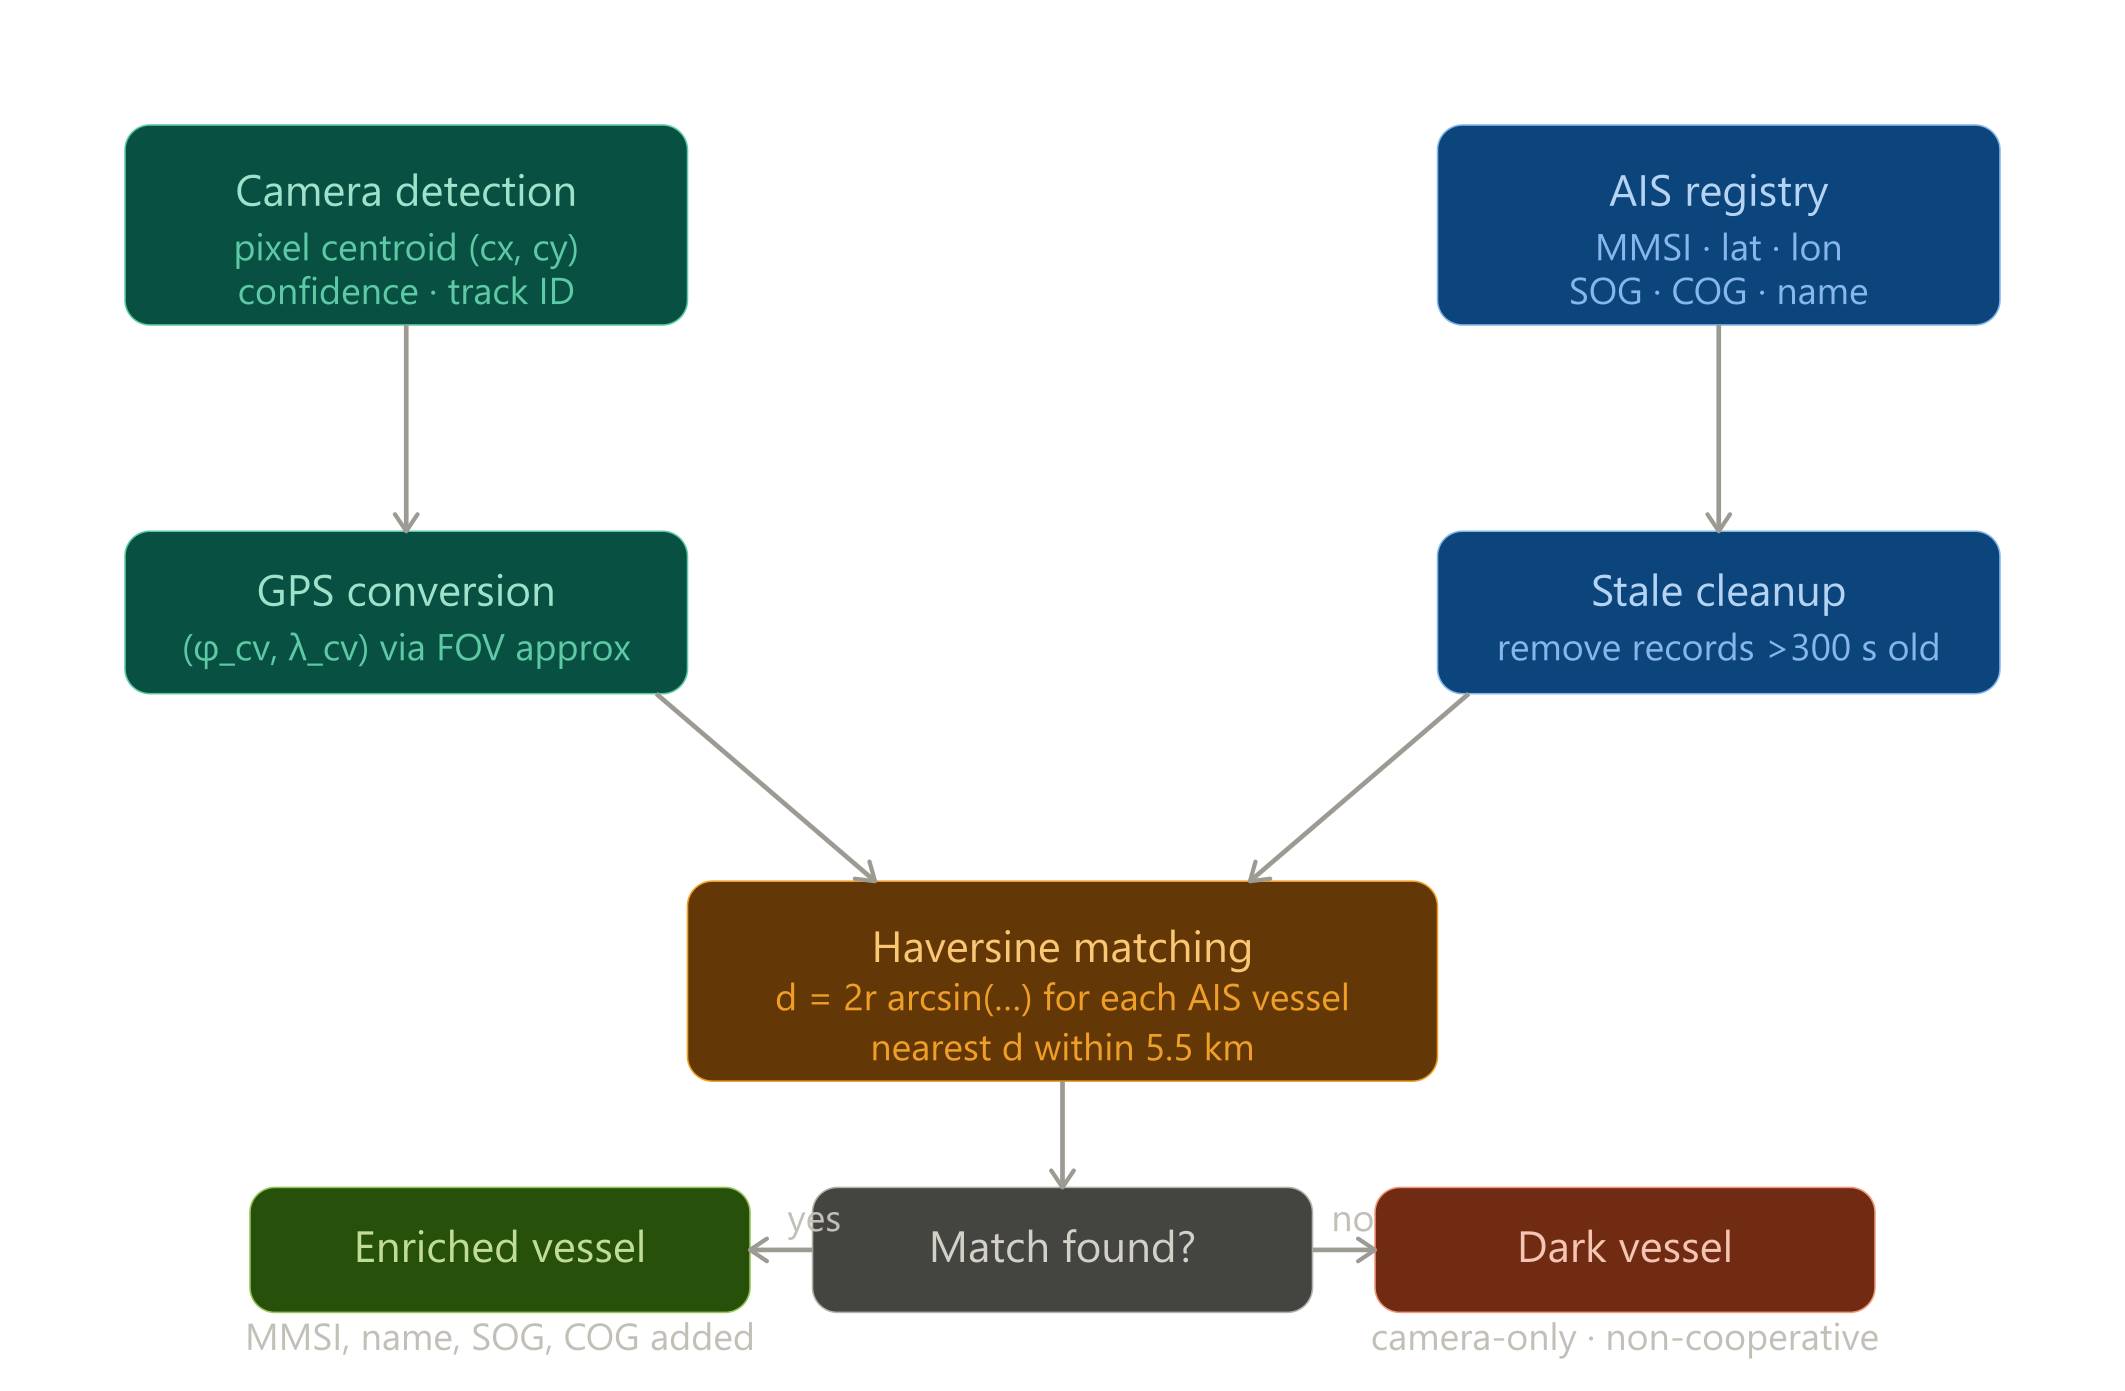
\includegraphics[width=0.95\textwidth]{Chapter4/Figures/cv_ais_fusion.png}
\caption{\gls{ais}--Computer Vision Data Fusion Process}
\label{fig:fusion}
\end{figure}

\subsection{LSTM Trajectory Prediction}

With a stable sequence of historical positions established, the data is routed to the trajectory prediction module. Because vessel movement is sequential and influenced by past maneuvers, an \gls{lstm} network was chosen over simpler regression models to capture these complex temporal dependencies.

The architecture comprises two stacked \gls{lstm} layers feeding into a fully connected output layer (Figure~\ref{fig:lstm}). The input at each timestep is a feature vector containing the vessel's latitude, longitude, \gls{sog}, sine and cosine encodings of the \gls{cog}, and a categorical vessel-type identifier. The network was trained on historical tracking data using \gls{mse} as the loss metric, optimized via the Adam algorithm. 

At runtime, the system slices the Kalman-filtered track history into fixed-length temporal windows and passes them through the trained model to forecast future coordinates. However, newly detected ships often lack sufficient historical data to fill the \gls{lstm}'s required input window. To prevent the pipeline from stalling, a kinematic linear regression fallback immediately takes over for these short-duration tracks, ensuring that the system always provides a predictive output regardless of track maturity.

\begin{figure}[H]
\centering
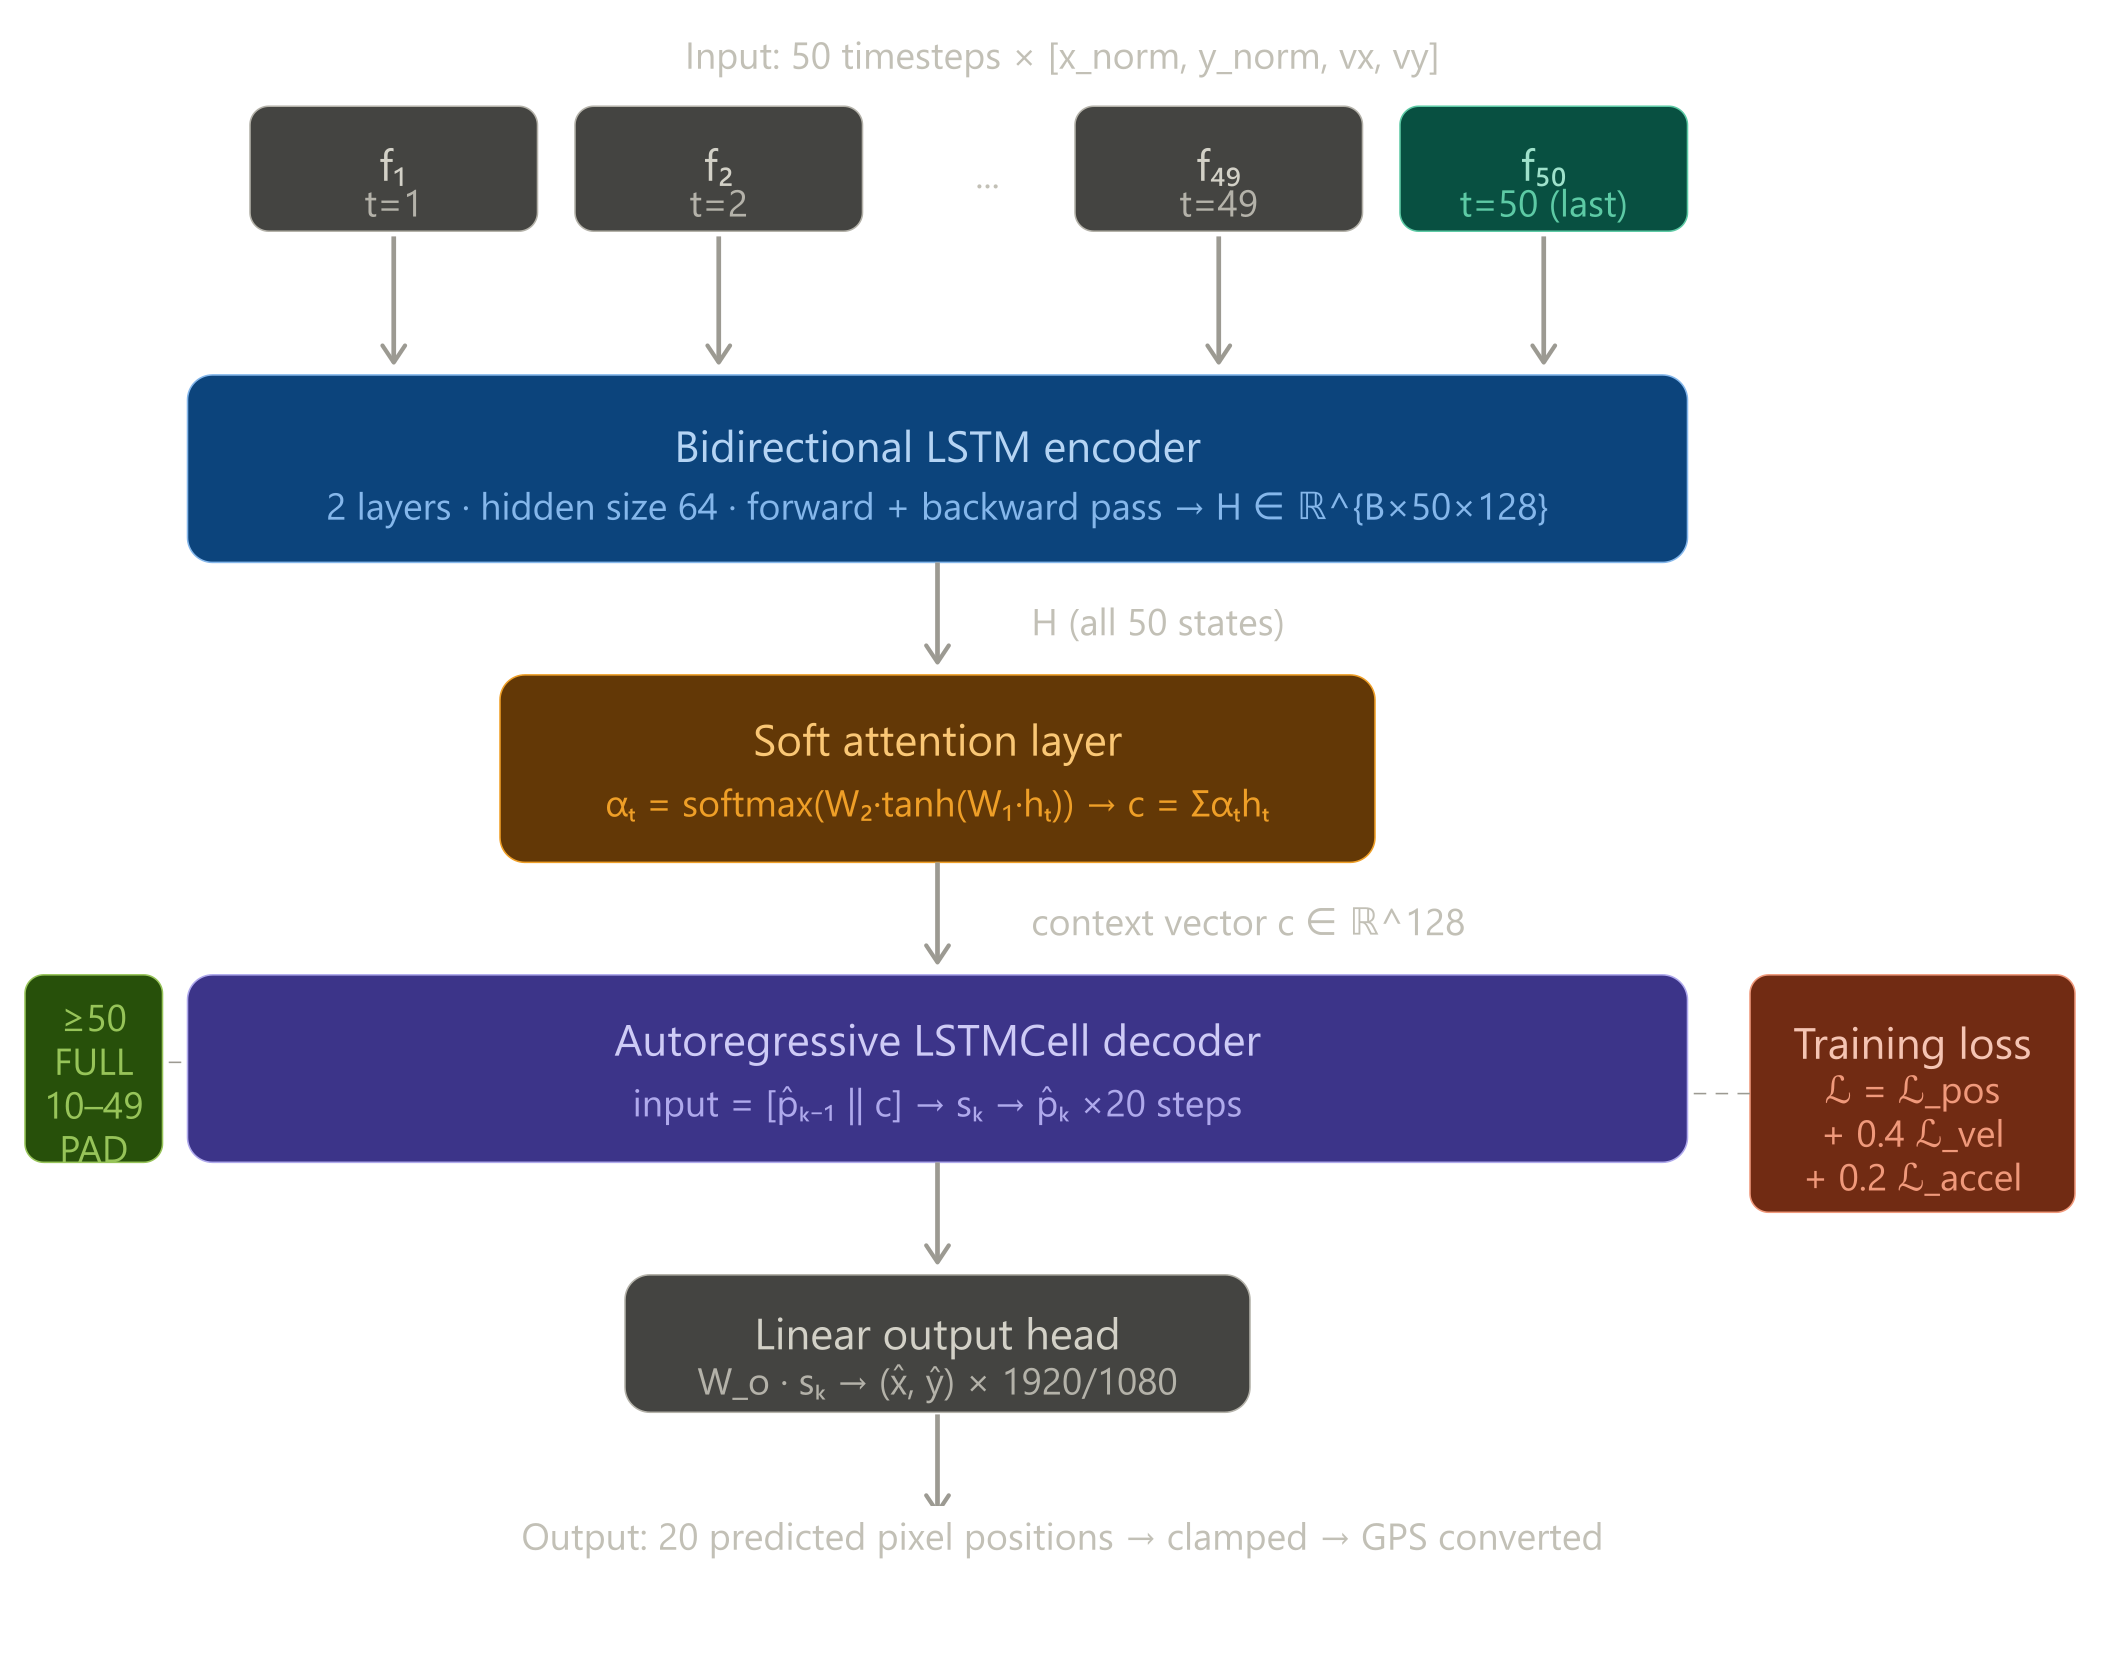
\includegraphics[width=0.90\textwidth]{Chapter4/Figures/lstm_architecture.png}
\caption{\gls{bilstm} Architecture for Vessel Trajectory Prediction}
\label{fig:lstm}
\end{figure}

\subsection{Geospatial Validation and Visualization}

Before the predicted trajectories are displayed to the user, they must pass through a land mask filter. This post-processing mechanism checks every forecasted coordinate against a global land-water topological map. If an \gls{lstm} prediction inadvertently routes a ship across a landmass—a common anomaly when predicting tight turns near coastlines—the filter intervenes, snapping the coordinate back to the nearest navigable water region. This guarantees physical realism in the system's output.

The finalized data is pushed to a dual-output visualization system. Using \gls{opencv}, bounding boxes, tracking IDs, speed annotations, and predicted paths are rendered directly onto the raw video feed for immediate visual confirmation. Concurrently, the geographical data is pushed to an interactive, Folium-based dashboard (Figure~\ref{fig:dashboard}). This web interface plots the live locations and forecasted trajectories on a global map, providing operators with comprehensive, real-time situational awareness.

\begin{figure}[H]
\centering
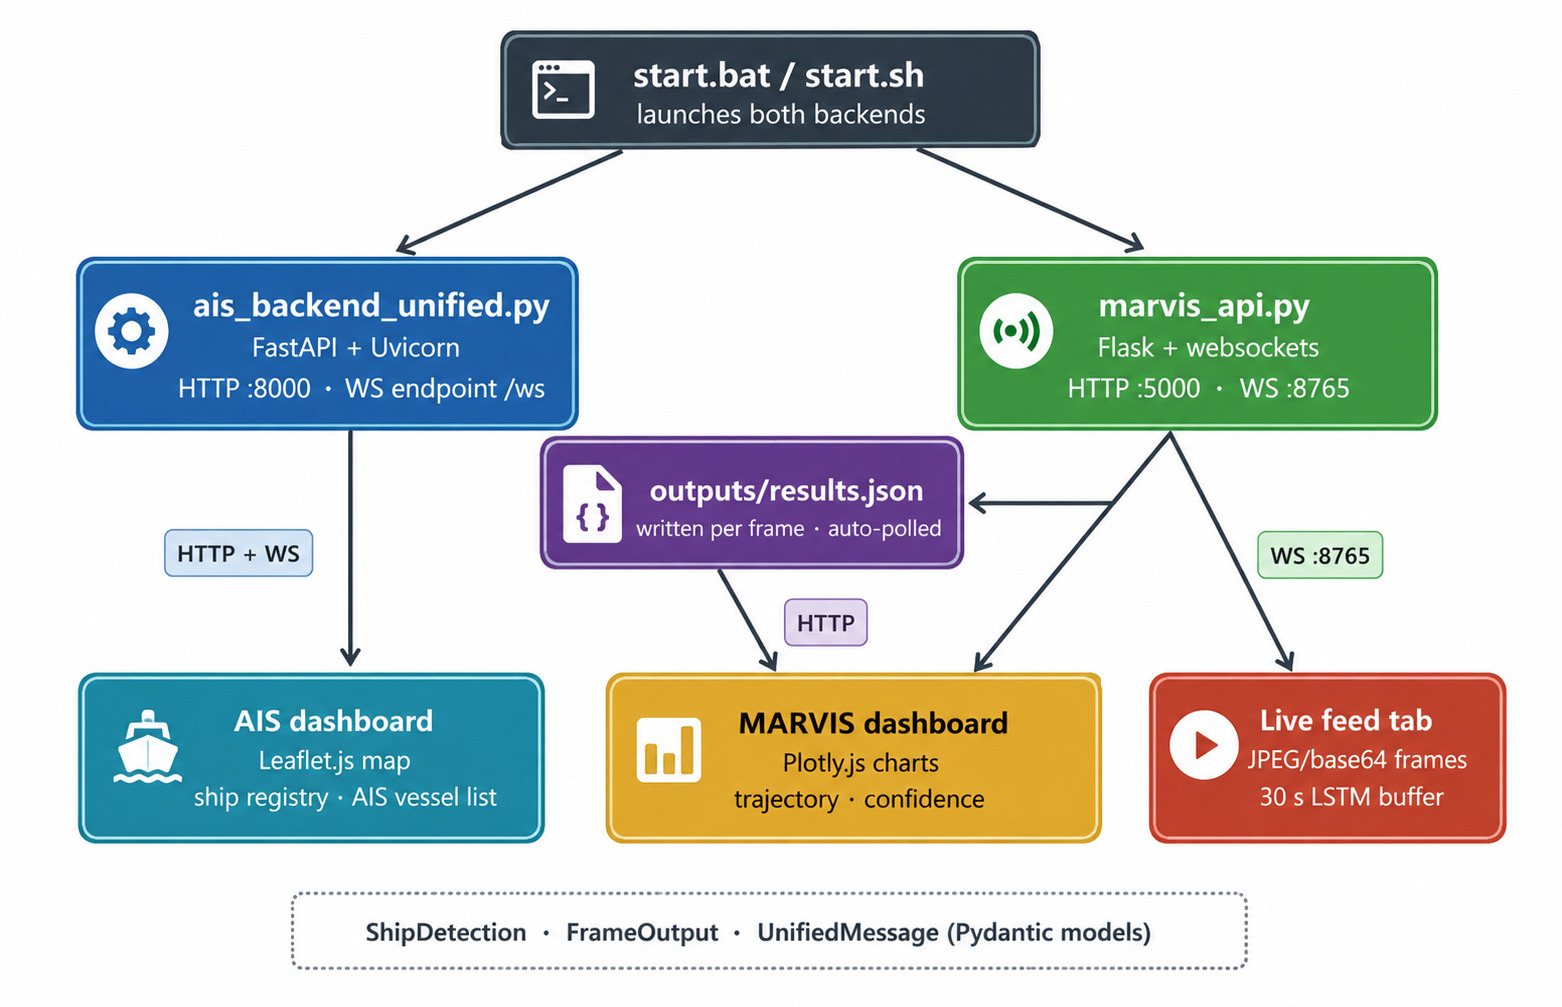
\includegraphics[width=0.95\textwidth]{Chapter4/Figures/dashboard_architecture.jpeg}
\caption{Dashboard Communication and Visualization Architecture}
\label{fig:dashboard}
\end{figure}

\section{Summary}

This chapter demonstrated how the theoretical designs from Chapter 3 were practically executed to build a functional, real-time surveillance pipeline. By establishing a \gls{cuda}-accelerated environment leveraging Python, \gls{pytorch}, and \gls{opencv}, the system successfully handles computationally intense deep learning tasks without sacrificing frame rate.

The data preparation phase established a robust 70:20:10 dataset used to fine-tune the \gls{yolov8} detector, which was seamlessly integrated with the \gls{deepocsort} tracker via \gls{osnet} appearance embeddings. By calculating inter-frame motion parameters and projecting them geographically, the pipeline successfully fuses live visual observations with \gls{ais} telemetry using Haversine nearest-neighbor matching and Kalman filtering. 

Finally, the implementation of the stacked \gls{lstm} network—supported by a kinematic regression fallback for new tracks and a land-mask filter for physical validation—ensures that the system generates highly accurate trajectory forecasts. These insights are ultimately routed to interactive \gls{opencv} and Folium dashboards, resulting in a cohesive, end-to-end framework whose performance metrics will be rigorously evaluated in the following chapter.
